\documentclass{ximera}

%\usepackage{todonotes}

\newcommand{\todo}{}

\usepackage{esint} % for \oiint
\ifxake%%https://math.meta.stackexchange.com/questions/9973/how-do-you-render-a-closed-surface-double-integral
\renewcommand{\oiint}{{\large\bigcirc}\kern-1.56em\iint}
\fi


\graphicspath{
  {./}
  {ximeraTutorial/}
  {basicPhilosophy/}
  {functionsOfSeveralVariables/}
  {normalVectors/}
  {lagrangeMultipliers/}
  {vectorFields/}
  {greensTheorem/}
  {shapeOfThingsToCome/}
  {dotProducts/}
  {partialDerivativesAndTheGradientVector/}
  {../productAndQuotientRules/exercises/}
  {../normalVectors/exercisesParametricPlots/}
  {../continuityOfFunctionsOfSeveralVariables/exercises/}
  {../partialDerivativesAndTheGradientVector/exercises/}
  {../directionalDerivativeAndChainRule/exercises/}
  {../commonCoordinates/exercisesCylindricalCoordinates/}
  {../commonCoordinates/exercisesSphericalCoordinates/}
  {../greensTheorem/exercisesCurlAndLineIntegrals/}
  {../greensTheorem/exercisesDivergenceAndLineIntegrals/}
  {../shapeOfThingsToCome/exercisesDivergenceTheorem/}
  {../greensTheorem/}
  {../shapeOfThingsToCome/}
  {../separableDifferentialEquations/exercises/}
  {vectorFields/}
}

\newcommand{\mooculus}{\textsf{\textbf{MOOC}\textnormal{\textsf{ULUS}}}}

\usepackage{tkz-euclide}
\usepackage{tikz}
\usepackage{tikz-cd}
\usetikzlibrary{arrows}
\tikzset{>=stealth,commutative diagrams/.cd,
  arrow style=tikz,diagrams={>=stealth}} %% cool arrow head
\tikzset{shorten <>/.style={ shorten >=#1, shorten <=#1 } } %% allows shorter vectors

\usetikzlibrary{backgrounds} %% for boxes around graphs
\usetikzlibrary{shapes,positioning}  %% Clouds and stars
\usetikzlibrary{matrix} %% for matrix
\usepgfplotslibrary{polar} %% for polar plots
\usepgfplotslibrary{fillbetween} %% to shade area between curves in TikZ
%\usetkzobj{all}
\usepackage[makeroom]{cancel} %% for strike outs
%\usepackage{mathtools} %% for pretty underbrace % Breaks Ximera
%\usepackage{multicol}
\usepackage{pgffor} %% required for integral for loops



%% http://tex.stackexchange.com/questions/66490/drawing-a-tikz-arc-specifying-the-center
%% Draws beach ball
\tikzset{pics/carc/.style args={#1:#2:#3}{code={\draw[pic actions] (#1:#3) arc(#1:#2:#3);}}}



\usepackage{array}
\setlength{\extrarowheight}{+.1cm}
\newdimen\digitwidth
\settowidth\digitwidth{9}
\def\divrule#1#2{
\noalign{\moveright#1\digitwidth
\vbox{\hrule width#2\digitwidth}}}




% \newcommand{\RR}{\mathbb R}
% \newcommand{\R}{\mathbb R}
% \newcommand{\N}{\mathbb N}
% \newcommand{\Z}{\mathbb Z}

\newcommand{\sagemath}{\textsf{SageMath}}


%\renewcommand{\d}{\,d\!}
%\renewcommand{\d}{\mathop{}\!d}
%\newcommand{\dd}[2][]{\frac{\d #1}{\d #2}}
%\newcommand{\pp}[2][]{\frac{\partial #1}{\partial #2}}
% \renewcommand{\l}{\ell}
%\newcommand{\ddx}{\frac{d}{\d x}}

% \newcommand{\zeroOverZero}{\ensuremath{\boldsymbol{\tfrac{0}{0}}}}
%\newcommand{\inftyOverInfty}{\ensuremath{\boldsymbol{\tfrac{\infty}{\infty}}}}
%\newcommand{\zeroOverInfty}{\ensuremath{\boldsymbol{\tfrac{0}{\infty}}}}
%\newcommand{\zeroTimesInfty}{\ensuremath{\small\boldsymbol{0\cdot \infty}}}
%\newcommand{\inftyMinusInfty}{\ensuremath{\small\boldsymbol{\infty - \infty}}}
%\newcommand{\oneToInfty}{\ensuremath{\boldsymbol{1^\infty}}}
%\newcommand{\zeroToZero}{\ensuremath{\boldsymbol{0^0}}}
%\newcommand{\inftyToZero}{\ensuremath{\boldsymbol{\infty^0}}}



% \newcommand{\numOverZero}{\ensuremath{\boldsymbol{\tfrac{\#}{0}}}}
% \newcommand{\dfn}{\textbf}
% \newcommand{\unit}{\,\mathrm}
% \newcommand{\unit}{\mathop{}\!\mathrm}
% \newcommand{\eval}[1]{\bigg[ #1 \bigg]}
% \newcommand{\seq}[1]{\left( #1 \right)}
% \renewcommand{\epsilon}{\varepsilon}
% \renewcommand{\phi}{\varphi}


% \renewcommand{\iff}{\Leftrightarrow}

% \DeclareMathOperator{\arccot}{arccot}
% \DeclareMathOperator{\arcsec}{arcsec}
% \DeclareMathOperator{\arccsc}{arccsc}
% \DeclareMathOperator{\si}{Si}
% \DeclareMathOperator{\scal}{scal}
% \DeclareMathOperator{\sign}{sign}


%% \newcommand{\tightoverset}[2]{% for arrow vec
%%   \mathop{#2}\limits^{\vbox to -.5ex{\kern-0.75ex\hbox{$#1$}\vss}}}
% \newcommand{\arrowvec}[1]{{\overset{\rightharpoonup}{#1}}}
% \renewcommand{\vec}[1]{\arrowvec{\mathbf{#1}}}
% \renewcommand{\vec}[1]{{\overset{\boldsymbol{\rightharpoonup}}{\mathbf{#1}}}}

% \newcommand{\point}[1]{\left(#1\right)} %this allows \vector{ to be changed to \vector{ with a quick find and replace
% \newcommand{\pt}[1]{\mathbf{#1}} %this allows \vec{ to be changed to \vec{ with a quick find and replace
% \newcommand{\Lim}[2]{\lim_{\point{#1} \to \point{#2}}} %Bart, I changed this to point since I want to use it.  It runs through both of the exercise and exerciseE files in limits section, which is why it was in each document to start with.

% \DeclareMathOperator{\proj}{\mathbf{proj}}
% \newcommand{\veci}{{\boldsymbol{\hat{\imath}}}}
% \newcommand{\vecj}{{\boldsymbol{\hat{\jmath}}}}
% \newcommand{\veck}{{\boldsymbol{\hat{k}}}}
% \newcommand{\vecl}{\vec{\boldsymbol{\l}}}
% \newcommand{\uvec}[1]{\mathbf{\hat{#1}}}
% \newcommand{\utan}{\mathbf{\hat{t}}}
% \newcommand{\unormal}{\mathbf{\hat{n}}}
% \newcommand{\ubinormal}{\mathbf{\hat{b}}}

% \newcommand{\dotp}{\bullet}
% \newcommand{\cross}{\boldsymbol\times}
% \newcommand{\grad}{\boldsymbol\nabla}
% \newcommand{\divergence}{\grad\dotp}
% \newcommand{\curl}{\grad\cross}
%\DeclareMathOperator{\divergence}{divergence}
%\DeclareMathOperator{\curl}[1]{\grad\cross #1}
% \newcommand{\lto}{\mathop{\longrightarrow\,}\limits}

% \renewcommand{\bar}{\overline}

\colorlet{textColor}{black}
\colorlet{background}{white}
\colorlet{penColor}{blue!50!black} % Color of a curve in a plot
\colorlet{penColor2}{red!50!black}% Color of a curve in a plot
\colorlet{penColor3}{red!50!blue} % Color of a curve in a plot
\colorlet{penColor4}{green!50!black} % Color of a curve in a plot
\colorlet{penColor5}{orange!80!black} % Color of a curve in a plot
\colorlet{penColor6}{yellow!70!black} % Color of a curve in a plot
\colorlet{fill1}{penColor!20} % Color of fill in a plot
\colorlet{fill2}{penColor2!20} % Color of fill in a plot
\colorlet{fillp}{fill1} % Color of positive area
\colorlet{filln}{penColor2!20} % Color of negative area
\colorlet{fill3}{penColor3!20} % Fill
\colorlet{fill4}{penColor4!20} % Fill
\colorlet{fill5}{penColor5!20} % Fill
\colorlet{gridColor}{gray!50} % Color of grid in a plot

\newcommand{\surfaceColor}{violet}
\newcommand{\surfaceColorTwo}{redyellow}
\newcommand{\sliceColor}{greenyellow}




\pgfmathdeclarefunction{gauss}{2}{% gives gaussian
  \pgfmathparse{1/(#2*sqrt(2*pi))*exp(-((x-#1)^2)/(2*#2^2))}%
}


%%%%%%%%%%%%%
%% Vectors
%%%%%%%%%%%%%

%% Simple horiz vectors
\renewcommand{\vector}[1]{\left\langle #1\right\rangle}


%% %% Complex Horiz Vectors with angle brackets
%% \makeatletter
%% \renewcommand{\vector}[2][ , ]{\left\langle%
%%   \def\nextitem{\def\nextitem{#1}}%
%%   \@for \el:=#2\do{\nextitem\el}\right\rangle%
%% }
%% \makeatother

%% %% Vertical Vectors
%% \def\vector#1{\begin{bmatrix}\vecListA#1,,\end{bmatrix}}
%% \def\vecListA#1,{\if,#1,\else #1\cr \expandafter \vecListA \fi}

%%%%%%%%%%%%%
%% End of vectors
%%%%%%%%%%%%%

%\newcommand{\fullwidth}{}
%\newcommand{\normalwidth}{}



%% makes a snazzy t-chart for evaluating functions
%\newenvironment{tchart}{\rowcolors{2}{}{background!90!textColor}\array}{\endarray}

%%This is to help with formatting on future title pages.
\newenvironment{sectionOutcomes}{}{}



%% Flowchart stuff
%\tikzstyle{startstop} = [rectangle, rounded corners, minimum width=3cm, minimum height=1cm,text centered, draw=black]
%\tikzstyle{question} = [rectangle, minimum width=3cm, minimum height=1cm, text centered, draw=black]
%\tikzstyle{decision} = [trapezium, trapezium left angle=70, trapezium right angle=110, minimum width=3cm, minimum height=1cm, text centered, draw=black]
%\tikzstyle{question} = [rectangle, rounded corners, minimum width=3cm, minimum height=1cm,text centered, draw=black]
%\tikzstyle{process} = [rectangle, minimum width=3cm, minimum height=1cm, text centered, draw=black]
%\tikzstyle{decision} = [trapezium, trapezium left angle=70, trapezium right angle=110, minimum width=3cm, minimum height=1cm, text centered, draw=black]


\title{Polynomials}

\begin{document}

\begin{abstract}
characteristics
\end{abstract}
\maketitle




\begin{definition} \textbf{\textcolor{green!50!black}{Polynomials}} 


Polynomial functions (over the real numbers) are functions that can be described as sums of power functions with whole number exponents.


\[    p(x) = a_n x^n + a_{n-1} x^{n-1} + \cdots + a_3 x^3 + a_2 x^2 + a_1 x^1 + a_0 x^0      \]

where the $a_k$ are real numbers and $a_n \ne 0$.


\begin{itemize}
\item Each of the summands is called a \textbf{term}.  
\item $n$ is called the \textbf{degree} of the polynomial.
\item $a_k$ are called \textbf{coefficients}.
\item $a_n$ is called the \textbf{leading coefficient}.
\item $a_n x^n$ is called the \textbf{leading term}.
\item $a_2 x^2$ is called the \textbf{quadratic term}.
\item $a_1 x^1$ is called the \textbf{linear term}, often written as $a_1 x$.
\item $a_0 x^0$ is called the \textbf{constant term}, often written as $a_0$.

\end{itemize}



This is called the \textbf{standard form}.
\end{definition}





For analytic purposes, we would prefer a product

\[   p(x) = a (x-r_n)(x-r_{n-1})  \cdots (x-r_2)(x-r_1)  \]


\begin{itemize}

\item $a$ is called the \textbf{leading coefficient}.
\item $(x-r_k)$ are called \textbf{factors}.
\item $r_k$ are called the \textbf{zeros} or \textbf{roots}.

\end{itemize}






Polynomials are the most familiar feeling functions we have. Their formulas look like extended linear or quadratic functions, just more terms.\\

The graph of $y = f(x) = \frac{1}{100} x^3 + \frac{1}{25} x^2 - \frac{31}{100} x - \frac{7}{10}$

\begin{image}
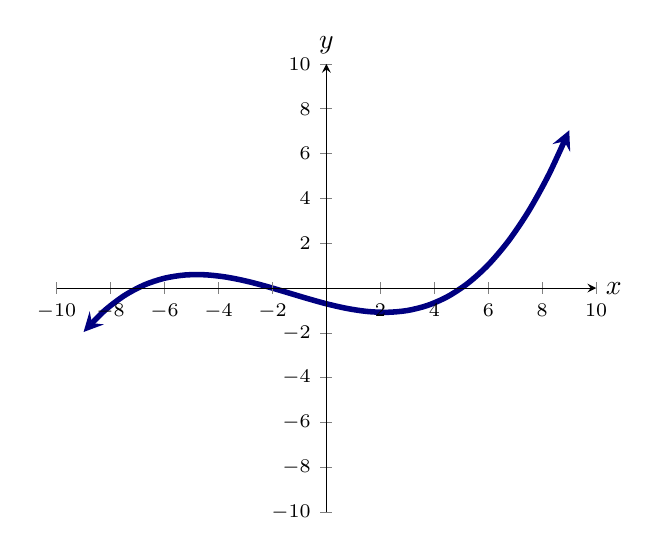
\begin{tikzpicture} 
  \begin{axis}[
            domain=-10:10, ymax=10, xmax=10, ymin=-10, xmin=-10,
            axis lines =center, xlabel=$x$, ylabel=$y$,
            ytick={-10,-8,-6,-4,-2,2,4,6,8,10},
            xtick={-10,-8,-6,-4,-2,2,4,6,8,10},
            ticklabel style={font=\scriptsize},
            every axis y label/.style={at=(current axis.above origin),anchor=south},
            every axis x label/.style={at=(current axis.right of origin),anchor=west},
            axis on top
          ]
          
          \addplot [line width=2, penColor, smooth, domain=(-9:9),<->] {0.01*(x+7)*(x+2)*(x-5)};

           

  \end{axis}
\end{tikzpicture}
\end{image}



All of the characteristics and features of polynomials are nice.

\begin{itemize}
\item Their domains include all real numbers. 
\item They are continuous everywhere.
\item No discontinuities or singularities.
\item No asymptotes on the graph.
\item Their graphs are smooth - no corners or endpoints
\end{itemize}


Polynomials smoothly alternate between increasing and decreasing, which switch at global and local maximums and minimums.

As you will see later, polynomials have a limit on the number of zeros and extrema they can have.  They cannot have more than the degree of the polynomial. So, what happens outside all of the wiggling?  This is known as the \textbf{end-behavior}.  All polynomials continue without bound after the zeros and extrema.  Either they tend to infinity or negative infinity, which is tied to the sign of the leading coefficient and the degree.
















\subsection*{Factored Form}


$p(x) = a (x-r_n)(x-r_{n-1})  \cdots (x-r_2)(x-r_1)$ is the \textbf{factored form} of a polynomial.  \\

In an effort to be clearer, we clean up the roots, because there could be repeated roots and we would like to point this out.  Therefore the reduced or simplified factored form looks like




\[   p(x) = a (x-r_n)^{e_n} (x-r_{n-1})^{e_{n-1}}  \cdots (x-r_2)^{e_2} (x-r_1)^{e_1}  \]



In this version, the $r_k$ are distinct roots.  They are all different. \\
The $e_k$ are the exponents and tell us how many times a particular root repeats.  The exponents are referred to as the factor's or the root's \textbf{multiplicity}.\\




\begin{definition} \textbf{\textcolor{green!50!black}{multiplicity}} 

Let $p(x)$ be a polynomial with root $r$.  The number of times $(x - r)$ appears in the complete factorization of $p(x)$ is called the \textbf{multiplicity} of $r$.

\end{definition}

As we saw with quadratics, this factorization into linear factors often requires complex numbers, which we will encounter later in this course. We are only using real numbers now.  Therefore, our factorizations will include linear factors as well as irreducible quadratic factors (nonreal roots).

\textbf{\textcolor{red!90!darkgray}{$\blacktriangleright$}}  Therefore, our discussion on polynomial roots, will center around the linear factors.  Irreducible quadratics will have to stay that way until the next course.










\textbf{\large Running the Number Line}

If we think of the real numbers as lining up to form the number line, then we could imagine ourselves running over the number line from $-\infty$ to $\infty$, or from left to right.  We would hit every real number once.  \\

For a polynomial, we would run through each distinct root once.  As we ran from the left side to the right side of each root, the sign of the value of the polynomial with either change or stay the same.

At each root, $r_k$, the value of the polynomial is $0$.  But on either side of the root, the polynomial is either positive or negative. There are four possible combinations.


\[
\begin{array}{rcl}
\text{Left of Root}  & \text{Root}  & \text{Right of Root} \\
positive & 0 & positive \\
negative & 0 & negative \\
positive & 0 & negative \\
negative & 0 & positive
\end{array}
\]


Either the sign switches or it stays the same across the root.  How can we see this in the formula?



\[   f(x) = a (x-r_n)^{e_n} (x-r_{n-1})^{e_{n-1}}  \cdots (x-r_2)^{e_2} (x-r_1)^{e_1}  \]


If we imagine ourselves running through $r_k$ in the domain, then $(x-r_k)^{e_k}$ is the only factor that could possibly change sign.  All of the other factors maintain their same sign when $x$ runs through $r_k$.



Let's examine the factor $(x-r_k)^{e_k}$:

As $x$ runs from less than $r_k$ to greater than $r_k$, the base of this factor changes from negative to positive:

\begin{itemize}
\item when $x<r_k$, then $x-r_k <0$.  \\

\item when $x>r_k$, then $x-r_k >0$. \\
\end{itemize}


If the exponent, $e_k$, is even, then the sign of $x-r_k$ doesn't matter. The sign of the whole factor $(x-r_k)^{e_k}$ will be positve regardless of the sign of the base.

However, if $e_k$ is odd then the sign of the base does matter, because, unlike an even power, a negative number raise to an odd power will remain negative.





\begin{itemize}
\item If $e_k$ is odd, then $(x-r_k)^{e_k}$ will change sign.
\item If $e_k$ is even, then $(x-r_k)^{e_k}$ will not change sign.
\end{itemize}







\begin{itemize}
\item If $r_k$ is a root of odd multiplicty, then $(x-r_k)^{e_k}$ will change sign as $x$ runs through $r_k$ in the domain.
\item If $e_k$ is a root of even multiplicty, then $(x-r_k)^{e_k}$ will not change sign as $x$ runs through $r_k$ in the domain.
\end{itemize}






\begin{example}


Let $p(x) = 3(x+4) (x-1)^2 (x-3)$.

$p$ has four different factors: $3$, $x+4$, $x-1$, and $x-3$.  The factor $3$ is always positive, but the other three factors might change signs over their corresponding zeros, which are $-4$, $1$, and $3$.


$\blacktriangleright$ \textbf{The $x+4$ factor:}

\begin{image}
  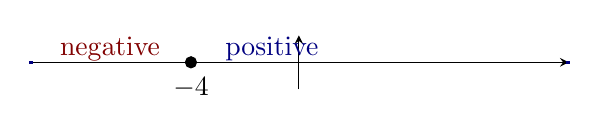
\begin{tikzpicture}
    \begin{axis}[
            %xmin=-25,xmax=25,ymin=-25,ymax=25,
            %width=3in,
            clip=false,
            axis lines=center,
            %ticks=none,
            unit vector ratio*=1 1 1,
            ymajorticks=false,
            xtick={-4},
            %xlabel=$x$, ylabel=$y$,
            %every axis y label/.style={at=(current axis.above origin),anchor=south},
            every axis x label/.style={at=(current axis.right of origin),anchor=west},
          ]     

            \addplot [color=black,only marks,mark=*] coordinates{(-4,0)};

            \addplot [line width=1, penColor, smooth,samples=100,domain=(-10:-9.9)] ({x},{0});
            \addplot [line width=1, penColor, smooth,samples=100,domain=(9.9:10)] ({x},{0});

            \node at (axis cs:-7,0.5) [penColor2] {negative};
            \node at (axis cs:-1,0.5) [penColor] {positive};



        \end{axis}
  \end{tikzpicture}
  \end{image}







$\blacktriangleright$ \textbf{The $x-1$ factor:}

\begin{image}
  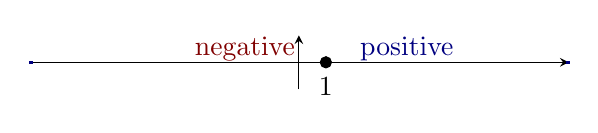
\begin{tikzpicture}
    \begin{axis}[
            %xmin=-25,xmax=25,ymin=-25,ymax=25,
            %width=3in,
            clip=false,
            axis lines=center,
            %ticks=none,
            unit vector ratio*=1 1 1,
            ymajorticks=false,
            xtick={1},
            %xlabel=$x$, ylabel=$y$,
            %every axis y label/.style={at=(current axis.above origin),anchor=south},
            every axis x label/.style={at=(current axis.right of origin),anchor=west},
          ]     

            \addplot [color=black,only marks,mark=*] coordinates{(1,0)};

            \addplot [line width=1, penColor, smooth,samples=100,domain=(-10:-9.9)] ({x},{0});
            \addplot [line width=1, penColor, smooth,samples=100,domain=(9.9:10)] ({x},{0});

            \node at (axis cs:-2,0.5) [penColor2] {negative};
            \node at (axis cs:4,0.5) [penColor] {positive};



        \end{axis}
  \end{tikzpicture}
  \end{image}

Except, this factor actually has an even exponent, which means the factors will not change signs over $1$.





$\blacktriangleright$ \textbf{The $(x-1)^2$ factor:}

\begin{image}
  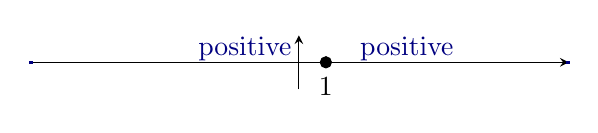
\begin{tikzpicture}
    \begin{axis}[
            %xmin=-25,xmax=25,ymin=-25,ymax=25,
            %width=3in,
            clip=false,
            axis lines=center,
            %ticks=none,
            unit vector ratio*=1 1 1,
            ymajorticks=false,
            xtick={1},
            %xlabel=$x$, ylabel=$y$,
            %every axis y label/.style={at=(current axis.above origin),anchor=south},
            every axis x label/.style={at=(current axis.right of origin),anchor=west},
          ]     

            \addplot [color=black,only marks,mark=*] coordinates{(1,0)};

            \addplot [line width=1, penColor, smooth,samples=100,domain=(-10:-9.9)] ({x},{0});
            \addplot [line width=1, penColor, smooth,samples=100,domain=(9.9:10)] ({x},{0});

            \node at (axis cs:-2,0.5) [penColor] {positive};
            \node at (axis cs:4,0.5) [penColor] {positive};



        \end{axis}
  \end{tikzpicture}
  \end{image}









$\blacktriangleright$ \textbf{The $x-3$ factor:}

\begin{image}
  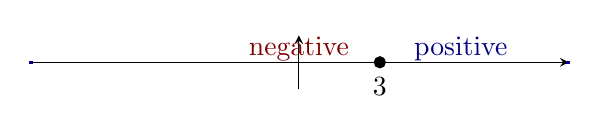
\begin{tikzpicture}
    \begin{axis}[
            %xmin=-25,xmax=25,ymin=-25,ymax=25,
            %width=3in,
            clip=false,
            axis lines=center,
            %ticks=none,
            unit vector ratio*=1 1 1,
            ymajorticks=false,
            xtick={3},
            %xlabel=$x$, ylabel=$y$,
            %every axis y label/.style={at=(current axis.above origin),anchor=south},
            every axis x label/.style={at=(current axis.right of origin),anchor=west},
          ]     

            \addplot [color=black,only marks,mark=*] coordinates{(3,0)};

            \addplot [line width=1, penColor, smooth,samples=100,domain=(-10:-9.9)] ({x},{0});
            \addplot [line width=1, penColor, smooth,samples=100,domain=(9.9:10)] ({x},{0});

            \node at (axis cs:0,0.5) [penColor2] {negative};
            \node at (axis cs:6,0.5) [penColor] {positive};



        \end{axis}
  \end{tikzpicture}
  \end{image}


The polynomial function has three zeros: $-4$, $1$, and $3$. \\

In between these zeros, the values of the polynomial function has a positive or negative sign. It can't change. \\

The sign of the whole polynomial depends on the \textbf{\textcolor{purple!85!blue}{product}} of the signs of the individual factors.



\begin{itemize}
\item For $x < -4$, 
\begin{itemize}
  \item $3 > 0$
  \item $x+4 < 0$
  \item $(x-1)^2 > 0$
  \item $x-3 < 0$ 
\end{itemize}
The whole polynomial is positive. We also know this because $p$ is a fourth degree polynomial and the leading coefficient is positive.


\item For $-4 < x < 1$, 
\begin{itemize}
  \item $3 > 0$
  \item $x+4 > 0$
  \item $(x-1)^2 > 0$
  \item $x-3 < 0$ 
\end{itemize}
The whole polynomial is negative. The also agrees with the fact that $p$ was positive and MUST change signs over $-4$, since we have an odd multiplicity.


\item For $1 < x < 3$, 
\begin{itemize}
  \item $3 > 0$
  \item $x+4 > 0$
  \item $(x-1)^2 > 0$
  \item $x-3 < 0$ 
\end{itemize}
The whole polynomial is negative. The also agrees with the fact that $p$ was negative and DOES NOT change signs over $1$, since we have an even multiplicity.


\item For $3 < x$, 
\begin{itemize}
  \item $3 > 0$
  \item $x+4 > 0$
  \item $(x-1)^2 > 0$
  \item $x-3 > 0$ 
\end{itemize}
The whole polynomial is positive. The also agrees with the fact that $p$ was negative and MUST change signs over $3$, since we have an odd multiplicity.
\end{itemize}










$\blacktriangleright$ \textbf{The whole polynomial $3(x+4)(x-1)^2(x-3)$}

\begin{image}
  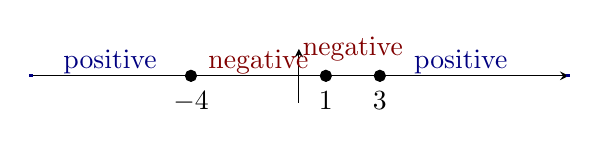
\begin{tikzpicture}
    \begin{axis}[
            %xmin=-25,xmax=25,ymin=-25,ymax=25,
            %width=3in,
            clip=false,
            axis lines=center,
            %ticks=none,
            unit vector ratio*=1 1 1,
            ymajorticks=false,
            xtick={-4,1,3},
            %xlabel=$x$, ylabel=$y$,
            %every axis y label/.style={at=(current axis.above origin),anchor=south},
            every axis x label/.style={at=(current axis.right of origin),anchor=west},
          ]     

            \addplot [color=black,only marks,mark=*] coordinates{(-4,0)};
            \addplot [color=black,only marks,mark=*] coordinates{(1,0)};
            \addplot [color=black,only marks,mark=*] coordinates{(3,0)};

            \addplot [line width=1, penColor, smooth,samples=100,domain=(-10:-9.9)] ({x},{0});
            \addplot [line width=1, penColor, smooth,samples=100,domain=(9.9:10)] ({x},{0});

            
            \node at (axis cs:-7,0.5) [penColor] {positive};
            \node at (axis cs:-1.5,0.5) [penColor2] {negative};
            \node at (axis cs:2,1.0) [penColor2] {negative};
            \node at (axis cs:6,0.5) [penColor] {positive};



        \end{axis}
  \end{tikzpicture}
  \end{image}




All of the information about the sign of the polynomial is encoded in the exponents. \\


Our polynomial here has a positive leading coefficient and is of degree $4$. Any fourth degree polynomial with a positive leading coefficient approaches $\infty$ as the domain approaches $-\infty$.  Our polynomial is positive for domain numbers less than $-4$.


Then, this polynomial must change signs at $-4$, because $-4$ has odd multiplicity.  Then, this polynomial cannot change signs at $1$, since it has even multiplicity.  Then, this polynomial must change signs at $3$.  Finally, any fourth degree polynomial with a positive leading coefficient approaches $\infty$ as the domain approaches $\infty$.
 


\end{example}

All of this should agree with the graph of the polynomial. \\
























\textbf{\textcolor{purple!85!blue}{Graphically}} 

Graphically, the values of the function are measured vertically. Zeroes are represented as dots positioned on the horizontal axis.  The graph either flows from one side of the horizontal axis to the other side as the function changes sign or the graph rebounds from the intercept and stays on the same side of the horizontal axis.  The multiplicity of the root tells us which.






\begin{example}

Change the exponent of the $x+2$ factor from odd to even.  The graph will crossover the $x$-axis for odd exponents and bounce back for even expoents.  If you change the sign of the leading coefficient, then the crossing and bouncing will jump to the other side of the $x$-axis.



\begin{center}
\desmos{igck8p6w15}{400}{300}
\end{center}

\end{example}






















\textbf{\textcolor{purple!85!blue}{Extrema}} 

Unless we have a quadratic polynomial, the best we can do for the maximums and minimums, at this point, is estimate them.







\begin{example}

The graph of $y = f(x) = 0.1(x+2)^3(x-3)$.



\begin{center}
\desmos{igck8p6w15}{400}{300}
\end{center}



$f(x)$ has an approximate global minimum value of $\answer[tolerance=0.1]{-6.6}$, which occurs approximately at $\answer[tolerance=0.1]{1.75}$.


\end{example}









\subsection*{Rate of Change}


Extending our analysis of quadratic functions, the global and local extreme values of a function occur at numbers in the domain where the corresponding points on the graph have horizontal tangent lines. We call these domain numbers \textbf{critical numbers}.  Thus, critical numbers play an important role in function analysis.  


It will take some further analysis to get a full definition of critical numbers. We'll start with critical numbers pointing out horizontal tangent lines in the graph and improve from there.









\begin{definition} \item \textbf{\textcolor{green!50!black}{Critical numbers}}

\textbf{Critical numbers} are domain numbers, which correspond to points on the graph where the tangent line has slope $0$ (is horizontal) or the tangent line has no slope (is vertical).

\end{definition}




Critical numbers are domain numbers marking flat/horizontal places in the graph.  These include tops of hills and bottoms of valleys. Critical numbers include places where extreme values occur.


The next example shows that they also include places that are not marking maximums or minimums.


















Polynomials are nice.  They increase and decrease on intervals defined by critical numbers marking places where the graph is horizontal and possible maximums and minimums.









\begin{example}

The graph of $y = f(x) = 0.1(x+2)^3(x-3)$.



\begin{center}
\desmos{qyzq162w2e}{400}{300}
\end{center}



$f$ has two critical numbers: $-2$ and $1.75$. These correspond to the two places where the graph has a horizontal tangent line.

\begin{itemize}
\item $f$ decreases on $\left(-\infty, \answer{1.75}\right]$.
\item $f$ increases on $\left[\answer{1.75}, \infty\right)$.
\end{itemize}




\end{example}


\textbf{Note:} $-2$ is a critical number, because the graph is flat there.  However, the sign of the rate of change of $f$ does not switch there, since $f$ does not have an extreme value there.










\subsection*{Zeros, Factors, and Intercepts}




Polynomial functions are nice.  They allow us to see many connections that we will keep in mind as we investigate other types of functions.


\textbf{\textcolor{red!90!darkgray}{$\blacktriangleright$}} Zeros, Factors, and Intercepts are different things but they all refer to the same idea.





\begin{itemize}

\item If $z_0$ is a zero of the polynomial $p(x)$, means $p(z_0)=0$.


\item If $(x-z_0)$ is a factor of the polynomial $p(x)$, means $p(x) = q(x) \cdot (x-z_0)$ for some polynomial $q(x)$.


\item If $(z_0,0)$ is an intercept of the graph of the polynomial $p(x)$, means $(z_0,0)$ is both on the horizontal axis and on the graph of $p$.

\end{itemize}


However, the existence of any of these implies the other two






\begin{itemize}

\item If $z_0$ is a zero of the polynomial $p(x)$, then $(x-z_0)$ is a factor and $(z_0,0)$ is on the graph.


\item If $(x-z_0)$ is a factor of the polynomial $p(x)$, then $p(z_0)=0$ and $(z_0,0)$ is on the graph.


\item If $(z_0,0)$ is an intercept of the graph of the polynomial $p(x)$, then $p(z_0)=0$ and $(x-z_0)$ is a factor.

\end{itemize}












\begin{onlineOnly}
\begin{center}
\textbf{\textcolor{green!50!black}{ooooo-=-=-=-ooOoo-=-=-=-ooooo}} \\

more examples can be found by following this link\\ \link[More Examples of Poynomial and Rational functions]{https://ximera.osu.edu/csccmathematics/precalculus/precalculus/polynomialFunctions/examples/exampleList}

\end{center}
\end{onlineOnly}



\end{document}
